%%%% Header %%%%%%%%%%%%%%%%%%%%%%%%%%%%%%%%%%%%%%%%%%%%%%%%%%%%%%%%%%%%%%%%%%%

\documentclass[12pt, parskip=half]{scrartcl}

\usepackage{jonas}

\bibliography{/home/jon/lucile/share/Dropbox/sci/refs/refs.bib}
\hyphenation{}

%%%% Meta data %%%%%%%%%%%%%%%%%%%%%%%%%%%%%%%%%%%%%%%%%%%%%%%%%%%%%%%%%%%%%%%%

\usepackage[
  pdfauthor   ={Jonas Schöley},
  pdftitle    ={The Gestational Age Pattern of Human Mortality},
  pdfsubject  ={},
  pdfkeywords ={},
  pdfproducer =Latex,
  pdfcreator  =pdflatex
]{hyperref}

\title{The Gestational Age Pattern of Human Mortality}
\author{
  Jonas Schöley\footnote{Max-Planck Odense Center on the Biodemography of Aging, University of Southern Denmark. Correspondence: \texttt{jschoeley@health.sdu.dk}.}
  \and
  James W.~Vaupel\footnote{Max-Planck Odense Center on the Biodemography of Aging, University of Southern Denmark. Max Planck Institute for Demographic Research, Rostock, Germany.}
  \and
  Rune Lindahl-Jacobsen\footnote{Max-Planck Odense Center on the Biodemography of Aging, University of Southern Denmark.}
  \and
  James Oeppen\footnote{Max-Planck Odense Center on the Biodemography of Aging, University of Southern Denmark.}
}

%%%% Titlepage %%%%%%%%%%%%%%%%%%%%%%%%%%%%%%%%%%%%%%%%%%%%%%%%%%%%%%%%%%%%%%%%

\begin{document}

\maketitle

\thispagestyle{empty}

\begin{abstract}
\textsc{Abstract.} In this study causes for \enquote{ontogenescense} -- the phenomenon of a declining force of mortality prior to maturity -- are analysed using data on human mortality by gestational age. Microdata on 4,018,830 births, fetal- and infant deaths in the United States of America in 2009 is used to calculate a joint fetal-infant life table by gestational age week 23 until week 100 after the last menstrual period of the mother. The joint life table has a remarkable regularity in the gestational age profile of fetal- and infant mortality: Mortality rates are declining over the whole observed age range with the exception of a \enquote{birth hump} peaking at week 38. The absolute rate of decline decreases over age. This observed gestational age pattern of the force of mortality is consistent with three hypotheses concerning the causes for ontogenescense: 1) Acquired robustness: as the organism growths it becomes more resilient towards death, 2) transitional timing: the transition of birth is a stressful event and momentarily increases the force of mortality, 3) mortality selection: The frailest individuals die first, resulting in the mean force of mortality to decline with age. In order to quantify the relative importance of these three processes a three component mortality model is fitted against the observed force of mortality. The model fits the data with high accuracy, suggesting that the phenomenon of ontogenescense in humans is fully explained by the three hypotheses or factors associated with these.
\end{abstract}

\clearpage

%%%% Text %%%%%%%%%%%%%%%%%%%%%%%%%%%%%%%%%%%%%%%%%%%%%%%%%%%%%%%%%%%%%%%%%%%%%

\section{Introduction} %%%%%%%%%%%%%%%%%%%%%%%%%%%%%%%%%%%%%%%%%%%%%%%%%%%%%%%%
\label{sec:introduction}

% The phenomenon of ontogenescense
Biologists noticed that for humans and many other species the instantaneous risk of death decreases from birth until onset of maturity (\cite{Medawar1952}, see \cite{Levitis2011} for a comprehensive literature review). This phenomenon is called \enquote{ontogenescence} and various hypotheses have been suggested for its explanation (see \cite{Levitis2011} for an overview). The aim of this study is to examine these hypotheses using data on human fetal- and infant mortality, with the ultimate goal of explaining the phenomenon of ontogenescence for humans.

% What we do in this paper and what question do we answer
Starting with the biological hypotheses on ontogenescense and using millions of individual level records on births, fetal- and infant deaths in the United States of America (US) a mathematical model of early life mortality is developed with the capacity to answer questions such as: How fast does a fetus/infant adapt to life? How risky is the transition of birth for the child? How important is mortality selection in explaining the aggregate age pattern of early life mortality? How heterogeneous is the fetal- population in terms of their mortality risk? Generally:

\begin{center}
  \emph{What drives the ontogenescent age decline of mortality?}
\end{center}

% Hypotheses on the causes for ontogenescense
\cite{Levitis2011} gives a comprehensive account of existing hypotheses attempting to explain the mechanisms driving the phenomenon of ontogenescense. The following list of hypotheses is adapted from \citeauthor{Levitis2011} review. We added the distinction between individual level and population level hypotheses and selected a primary reference for each hypothesis.

1.~\emph{Individual level explanations:} The mortality decline over age observed on a population level is thought to originate from a declining hazard of death of each individual organism. Examples of individual level hypotheses are:
  \emph{Growth-trade-off:} There is a trade-off between the current rate of growth and the current survival of an organism. Juvenile organisms who invest in fast growth momentarily worsen their survival chances with the prospect of increasing their adult survival once they have grown large (e.\,g.~\cite{Chu2008}).
  \emph{Acquired Robustness:} As an individual growths in becomes more resilient towards death (e.\,g.~\cite{Munch2006}).
  \emph{Transitional timing:} As the organism grows it has to pass a series of critical transitions, potentially dying at each. These transitions are concentrated early in life and therefore the mortality risk is concentrated in early life (\cite{Levitis2011}).

2.~\emph{Population level explanations:} The mortality decline over age is caused by mortality selection:\footnote{Within this article I relate the term \enquote{selection} solely to mortality without any implications for inheritance of specific traits as would be implied by its Darwinian meaning.} On average, the frailest individuals die first while the stronger individuals survive. Therefore, on the population level, the mean risk of death decreases over age. The \emph{Heterogeneous frailty} hypotheses (e.\,g.~\cite{Vaupel1985}) is an example for a population level hypothesis with a strong mathematical underpinning. A more specific example is \emph{Quality control:} the frailest die first, terminated by their kin (\cite{Hamilton1966}).

% The majority of these hypotheses are originating from biology and are supposed to explain ontogenescence for all kinds of life, not only for humans. Dealing with the specific case of ontogenescense in present day humans we can make additional assumptions which rule out some hypotheses from the start: 1.~

The questions is: Which of these hypotheses is supported by observations on present day humans being born into a modern health care system?

\section{Data and Methods} %%%%%%%%%%%%%%%%%%%%%%%%%%%%%%%%%%%%%%%%%%%%%%%%%%%%
\label{sec:data_and_methods}

% A joint fetal-infant life table from individual level data
The vital statistics of the US (births, deaths) are designated for public use. The data is extensive and thus allows for the detailed statistical analysis employed in this study. The analysis is based on individual births (N = 4,001,522), infant deaths (N = 18,923) and fetal deaths (N = 17,308) in the conception cohort 2009.\footnote{The data is derived from the \enquote{US Birth Cohort Linked Birth - Infant Death Data Files} and the \enquote{Fetal Death Data Files} for the years 2009 and 2010 (\cite{DVS2015})} The fetal death file does \emph{not} include cases of induced abortions limiting the data analysis to \emph{natural} causes of death for the pre-natal period. Using the Kaplan-Meier estimator life table survival functions are estimated. Two separate life tables are produced: 1) \emph{Infant mortality by day of age} from birth until 365 days after birth, and 2) \emph{joint fetal- and infant mortality by week of gestation} from week 23 to week 100 of gestation.

% Justifying the use of a joint fetal-infant life table
The reasons for joining fetal- and infant mortality are manifold: The gestational age pattern of mortality for joint fetal- and infant deaths are very regular which lend them to statistical analysis. Furthermore, the theory on ontogenescense is not limited to the time after birth. In fact \textcite{Levitis2011} shows a rough estimate of daily human mortality rates from conception until the $12^{th}$ birthday in the context of discussing \enquote{the evolutionary demography of ontogenesis}. Therefore using only half of the available data (either on infant- or on fetal- deaths) would be an arbitrary limitation. Using gestational age instead of demographic age also has the advantage of making a major source of unobserved heterogeneity in early life mortality observable: The different gestational ages at birth.

% Analysis
The final model of the gestational age pattern of human mortality is informed by the theory on ontogenescense and by an exploratory analysis of human infant- and joint fetal-infant mortality. In a first step of analysis life table mortality rates for infants over age are plotted. The hypotheses on ontogenescense are compared with the observed mortality pattern to identify promising candidates. The same exercise is then repeated with the observed mortality pattern of the joint fetal-infant life table over gestational age. This explorative analysis aims to inform the formal model of the \emph{gestational age pattern of human mortality}. This model is then formulated and fitted against the life table mortality rates using Poisson-maximum-likelihood estimation.

\section{The Age Pattern of Present US Infant Mortality} %%%%%%%%%%%%%%%%%%%%%%
\label{sec:the_daily_age_pattern_of_present_day_us_infant_mortality}

\begin{figure}[!htb]
  \begin{subfigure}[t]{0.5\textwidth}
    \centering
    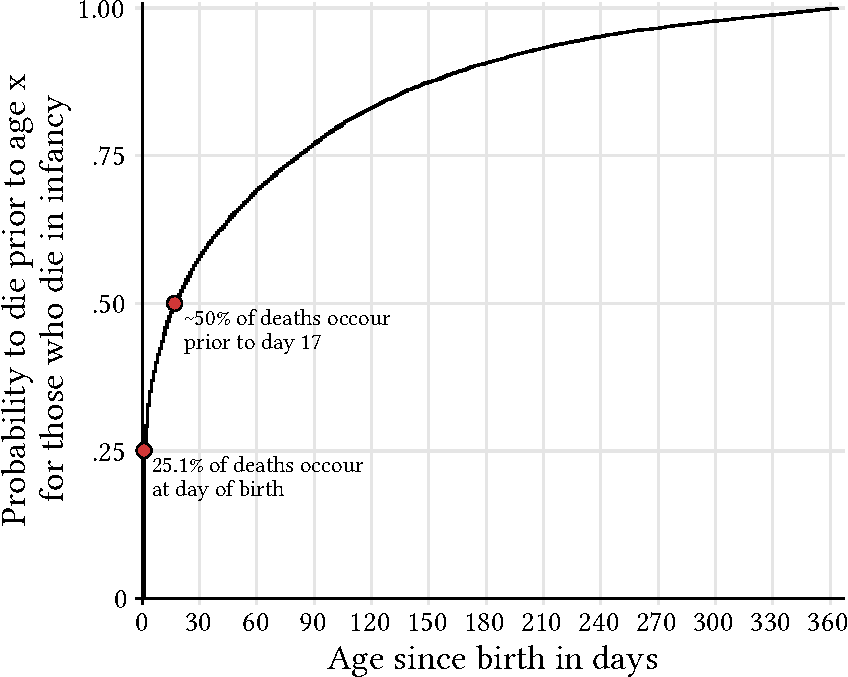
\includegraphics[width = \textwidth]{./fig/us_imort_2009_cumdx.pdf}
    \subcaption{Cumulative age distribution of infant deaths.}
    \label{fig:us_imort_2009_cumdx}
    \end{subfigure}%
  ~
    \begin{subfigure}[t]{0.5\textwidth}
    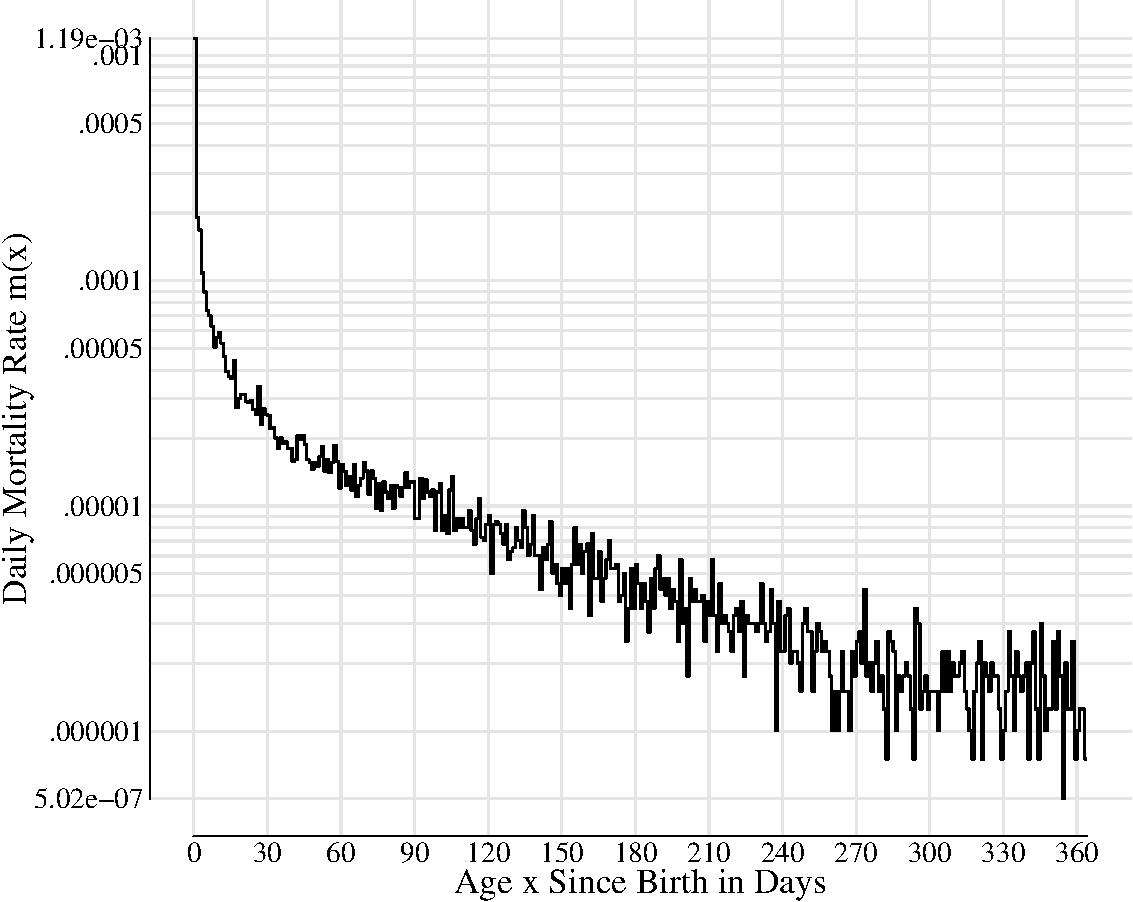
\includegraphics[width = \textwidth]{./fig/us_imort_2009_log_mx.pdf}
    \subcaption{Mortality rates over age during infancy.}
    \label{fig:us_imort_2009_log_mx}
    \end{subfigure}%
    \caption{Life-table characteristics of infant mortality for US infants conceived in 2009. Individual level data source: \cite{DVS2015}.}
    \label{fig:us_imort_2009}
\end{figure}

% Perinatal mortality
The absolute majority of the infant mortality risk is concentrated at the day of birth (see figure \ref{fig:us_imort_2009}). Of all observed infant deaths for the US conception cohort 2009, 25.1\,\% occur at the day of birth and half of them within the first 17 days of life. The infant mortality is clustered in the postpartum period. This supports two hypotheses:
\begin{inparaenum}
  \item \emph{transitional timing:} Birth is a high risk transition and temporarily increases an individuals mortality risk.
  \item \emph{heterogeneity:} Birth is a strong selector and selects the frailest individuals out of the population.
\end{inparaenum}
While there are many possible sources for unobserved heterogeneity regarding the risk of death, a major contribution may be the heterogeneity in gestational ages at birth. Age is defined as time since birth. This definition is ignorant to the fact that infants are born at different times after conception. We know that mortality risk is highly dependent on the gestational age at birth. The lower the gestational age, the lower the ability to survive the transition of birth (e.\,g.~\cite{Lubchenco1972}, \cite{Draper1999}). Therefore, in paediatric contexts, a different measure of time is commonly used: The \emph{gestational age}, defined as weeks since the last manse (e.\,g.~\cite{AAPCFN2004}).

% The trauma of birth
Compressing these thoughts into a single sentence it can be hypothesized that \emph{birth gives shape to the age pattern of infant mortality by momentarily increasing the risk of death for every individual and by selecting the frailest individuals out of the population.}

% Postpartum mortality
While neonatal mortality seems to be dominated by the trauma of birth, what is seen in mortality after the first month of age? Due to the large reduction in infant mortality we rarely see deaths after the postpartum period in the data. Still, an age pattern is present: Starting approximately at 50 days of chronological age the decline in infant mortality follows an exponential decay (see figure \ref{fig:us_imort_2009_log_mx}). This finding can be interpreted as a sign for \emph{acquired robustness}: The growth-rate of a child is the highest right after birth and declines from there on. If we assume that level of growth and level of mortality are inversely related, then the largest decline in mortality will fall into the period of the fastest growth, resulting in a negative exponential form of mortality decline due to growth.\footnote{The negative exponential shape of infant mortality is famously specified in the Siler model (\cite{Siler1979}).}

% Features of infant mortality
To summarise: we hypothesize that infant mortality can be explained as the sum of three components:
\begin{compactenum}
  \item The exponential decrease of mortality after 50 days of age is explained by \emph{acquired robustness} due to growth,
  \item the mortality outlier at the day of birth is explained by \emph{transitional timing} -- the added stress due to the struggle of birth, and
  \item the super-exponential decrease of mortality right after birth is explained by \emph{selection} against the most frail.
\end{compactenum}

\section{The Gestational Age Pattern of US Mortality} %%%%%%%%%%%%%%%%%%%%%%%%%
\label{sec:the_gestational_age_transformation}

% Justifying the gestational age scale
From a statistical point of view, the clustering of the majority of mortality risk in a single data point is problematic. We cannot learn much about the age pattern of infant mortality and of its components if the bulk of the variability is contained between two points: day 0 and day 1 after birth. Therefore we propose to look at mortality across the \emph{gestational age scale}. This scale transformation changes interpretation and shape of the mortality data in advantageous ways: Different gestational ages at birth are eliminated as a source of unobserved heterogeneity and the risky transition of birth is distributed along the time axis instead of clustered at the start. Because most fetal deaths occurring during the first half of the pregnancy are undetected and/or unreported we condition our population upon surviving to the $23^{rd}$ week of gestational age. From then on the vast majority of fetal deaths are believed to be registered.

% The gestational age pattern of human mortality
The human gestational age pattern as seen on our data has a very distinctive shape (see figure \ref{fig:us_fimort_2009_mx}). Mortality is highest at the start of the observation window and continuously decreases with a declining rate of change until the end of observation, only to be disrupted by a \emph{\enquote{birth hump}}. It seems that the \emph{birth spike} we can observe in infant mortality over age spread out into a distribution closely following the distribution of gestational ages at onset of labour. This can be explained on the population level: The higher the probability of birth at a given gestational age $x$, the higher the contribution of the stress at birth to the population hazard.

% Consistency of the human gestational age pattern with the theory
Overall, the data is consistent with what we see in infant mortality and the \emph{acquired robustness}, \emph{transitional timing} and \emph{selection} hypothesis continue being sensible choices for a final model.

\begin{figure}[!htb]
  \centering
  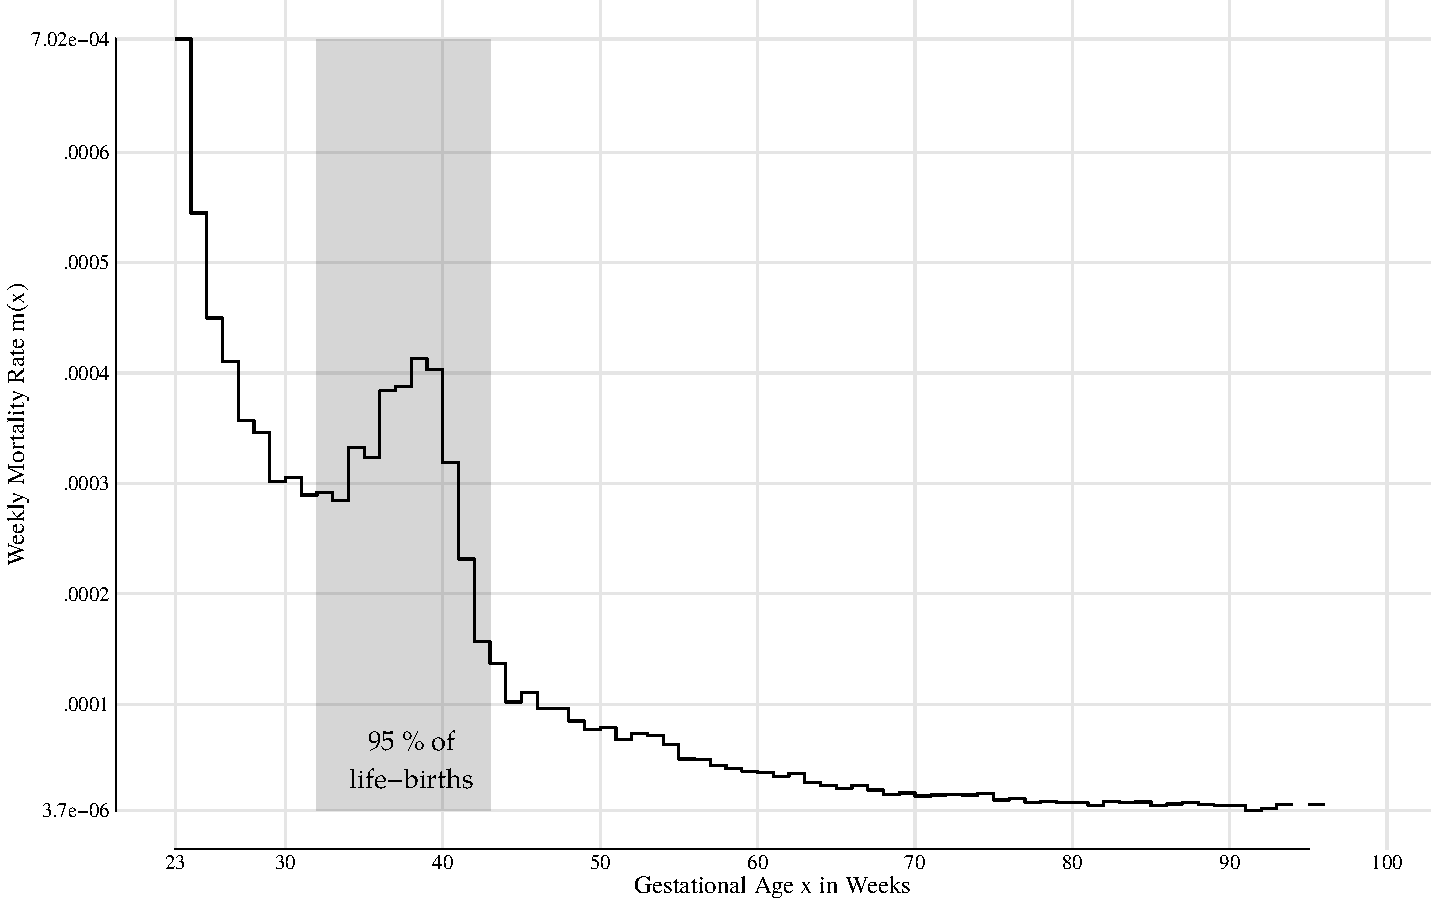
\includegraphics[width = \textwidth]{./fig/us_fimort_2009_mx.pdf}
  \caption{The gestational age pattern of human mortality for US fetus and infants conceived in 2009. Individual level data source: \cite{DVS2015}.}
  \label{fig:us_fimort_2009_mx}
\end{figure}

\section{A Model of Gestational Age Mortality} %%%%%%%%%%%%%%%%%%%%%%%%%%%%%%%%
\label{sec:modelling_the_gestational_age_pattern_of_human_mortality}

We identified three mechanisms that are consistent with data on the age pattern of infant mortality as well as with data on the gestational age pattern of human mortality:
\begin{inparaenum}
  \item \emph{Acquired robustness} as increasing resilience towards death due to growth,
  \item \emph{transitional timing} as the added stress due to the struggle of birth, and
  \item \emph{selection} as the early death of the frailest.
\end{inparaenum}
The task is to specify and formalize these hypotheses so that they can be checked against the data using a quantitative model.

We derive the aggregate model from the individual level. Let $i$ be an individual which survived until week 23 after the last manse of the mother. At any subsequent age\footnote{For mathematical convenience age $x$ in our model is defined as time passed since week 23 after the last manse of the mother. This is a straightforward transformation of the gestational age. To reverse it the gestational age origin (in our case 23 weeks) has to be added back to $x$.} $x$ the individual has an instantaneous risk of death $\mu_i(x)$. This risk changes as the individual grows older. From some initial level $\alpha_1$ at $x = 0$ it decreases with a constant relative rate $\lambda$ due to \emph{acquired robustness}. We model this process as

\begin{equation}
  \mu_i(x) = \alpha_1 e^{-\lambda x}.
  \label{eq:robust}
\end{equation}

At age $t_i$ labour sets in and the individual experiences a momentary increase of its risk of death because of the stressful and transitional nature of birth. We assume an additive and constant \emph{birth trauma} component $\alpha_2$ altering equation \ref{eq:robust} to

\begin{equation}
  \mu_i(x|t_i) =
  \begin{cases}
    \alpha_1 e^{-\lambda x} & x \neq t_i \\
    \alpha_1 e^{-\lambda x} + \alpha_2 & x = t_i \\
  \end{cases}.
  \label{eq:robustbirth}
\end{equation}

Setting the stage for the mortality selection effect on the aggregate level we assign a \emph{frailty}\footnote{See \cite{Vaupel1979} for the original formulation of the frailty model; see \cite{Wienke2011} for a general introduction to frailty models.} factor $z_i$ to each individual. This measure of an individuals susceptibility to death acts multiplicative and age-invariant on the risk of death. The lower the frailty factor of an individual the higher the individuals survival chances at any age. We extend equation \ref{eq:robustbirth} to

\begin{equation}
  \mu_i(x|t_i,z_i) =
  \begin{cases}
    z_i \cdot \alpha_1 e^{-\lambda x} & x \neq t \\
    z_i \cdot \alpha_1 e^{-\lambda x} + \alpha_2 & x = t \\
  \end{cases}.
  \label{eq:indhzrd}
\end{equation}

This expression completes our model of an \emph{individuals} mortality trajectory over gestational age. It looks quite different from the observed population hazard we showed in figure \ref{fig:us_fimort_2009_mx}, featuring a birth \emph{spike} instead of a \emph{hump} and lacking super-exponential decrease. Both these phenomena are thought to be exclusive to the population level and produced by aggregating over \emph{heterogeneous} individual trajectories. Differences between individuals are assumed to exist only in their \emph{frailty} $z_i$ and their age at the onset of labour $t_i$. Both are realizations of the random variables $Z$ and $T$ with probability densities $f_Z(z)$ and $f_T(t)$. Accordingly the the part of the age specific hazard that does not change between individuals, the \emph{baseline hazard} $\mu_0(x)$ is

\begin{equation}
  \mu_0(x) = \alpha_1 e^{-\lambda x}.
  \label{eq:baselinehzrd}
\end{equation}

As individuals with a high frailty have higher mortality and therefore shorter life-expectancy compared to those with a low frailty the the age specific average frailty in the population $E[f_Z(z|x)]$ is declining over age. This \emph{selection} effect produces a super-exponentially decreasing population level hazard $\overline{\mu}(x)$ even if individual hazards are declining exponentially.\footnote{This is on of the many \emph{ruses of heterogeneity} discussed in \cite{Vaupel1985}.} In the frailty model the population hazard is defined as the expected hazard in the population at age $x$. We write

\begin{equation}
  \overline{\mu_A}(x) = E[f_Z(z|x)] \times \mu_0(x).
  \label{eq:pophzrd_frailty1}
\end{equation}

So the population hazard component of our model accounting for selection and acquired robustness is given by

\begin{equation}
  \overline{\mu_A}(x) = E[f_Z(z|x)] \times \alpha_1 e^{-\lambda x}.
  \label{eq:pophzrd_frailty2}
\end{equation}

The \emph{birth hump} arises as an aggregation effect from differences in the timing of labour at the individual level. While the onset of labour is most likely at an gestational age of 38--42 weeks it might happen before and after. If onset of labour is rare at an age $x$ the added risk due to it will not change the population hazard (the average of the individual hazards) by much. Complementary, the more people experience labour at age $x$ the more this added momentary risk will show up in the population hazard. A distribution of individual-level \emph{birth spikes} turns into a single aggregate-level \emph{birth hump} which represents the added risk of birth for each individual $\alpha_2$ weighted by by the distribution of ages at onset of labour $f_T(t)$, resulting in

\begin{equation}
  \overline{\mu_B}(x) = \alpha_2 f_T(t),
\end{equation}

the birth trauma component of the population hazard.

Adding $\overline{\mu_A}(x)$ and $\overline{\mu_B}(x)$ completes the derivation of the aggregate level model from the individual level processes. We arrive at

\begin{equation}
  \underbrace{
    \overline{\mu}(x)
  }_{\substack{
    \text{Population hazard}\\ \text{at gestational age}~x
  }} =
  \underbrace{
    E[f_Z(z|x)]
  }_{\substack{
    \text{Average frailty}\\ \text{in population}\\ \text{at gestational age}~x
  }} \times
  \underbrace{
    \alpha_1 e^{-\lambda x}
  }_{\substack{
    \text{Acquired robustness}\\ \text{component of hazard}\\ \text{at gestational age}~x
  }} +
  \underbrace{
    \alpha_2 f_T(t).
  }_{\substack{
    \text{Birth trauma component}\\ \text{of hazard}\\ \text{at gestational age}~x.
  }}
  \label{eq:themodel}
\end{equation}

Lacking prior knowledge on the distribution of frailties at week 23 we follow \cite{Vaupel1979} in choosing the Gamma distribution with a unity mean for reasons of flexibility and traceability. Combining Gamma frailty with an exponential baseline hazard results in the well-known \emph{Gamma-Gompertz} model.\footnote{See \cite{Vaupel2014} for a recent discussion of the Gamma-Gompertz model.} Therefore

\begin{equation}
  E[f_Z(z|x)] \times \alpha_1 e^{-\lambda x} = \frac {\alpha_1 e^{-\lambda x}} {\frac{\gamma \alpha_1} {-\lambda} (e^{-\lambda x} - 1) + 1},
  \label{eq:gammagompertz}
\end{equation}

where $\gamma$ is the variance of the frailties in the population at the beginning of observation.

If the distribution of gestational ages at onset of labour $f_T(t)$ is not given in the data it has to be estimated. Analyses of hospital data show that $f_T(t)$ is skewed to the left and truncated to the right with a mode at around a gestational age of 40 weeks (\cite{Gardosi1997}). While preterm deliveries can stretch into the second trimester of pregnancy, labour is usually induced at postterm (>42 weeks of gestation). The \emph{scaled Beta} distribution (\cite{Johnson1995}) has the required features to model this situation. It is continuous, can be left tailed, and can be scaled over an arbitrary domain (in our case gestational age week 23 ($x = 0$) until week 47 ($x = 24$ weeks) -- the week of the last registered delivery in the data). The distribution of the gestational age at onset of labour has the form

\begin{equation}
  f_T(t) = \frac{1}{B(s_1,s_2)} \cdot \frac{x^{s_1-1} (24-x)^{s_2-1}} {24^{s_1+s_2-1}},
  \label{eq:beta}
\end{equation}

with $B(s_1,s_2)$ being the Beta function. The complete model has 6 free parameters:

\begin{tabular}{ll}
  $\alpha_1$ & The initial mortality level (at week 23 and process time 0). \\
  $\lambda$ & The relative rate of mortality decline over age. \\
  $\gamma$ & The initial variance of frailties in the population (at week 23 and process time 0).\\
  $\alpha_2$ & The added mortality risk due to the stress of birth. \\
  $s_1$ & The modal gestational age at onset of labour (in weeks after week 23). \\
  $s_2$ & The shape of the age distribution at onset of labour. \\
\end{tabular}

Substituting (\ref{eq:beta}) and (\ref{eq:gammagompertz}) in (\ref{eq:themodel}) yields the following \emph{law of mortality}:

\begin{equation}
  \overline{\mu}(x) =
  \frac {\alpha_1 e^{-\lambda x}} {\frac{\gamma \alpha_1} {-\lambda} (e^{-\lambda x} - 1) + 1} +
  \frac{\alpha_2 x^{s_1-1} (24-x)^{s_2-1}} {B(s_1,s_2) \cdot 24^{s_1+s_2-1}}.
  \label{eq:thelaw}
\end{equation}

\begin{figure}[!htb]
  \centering
  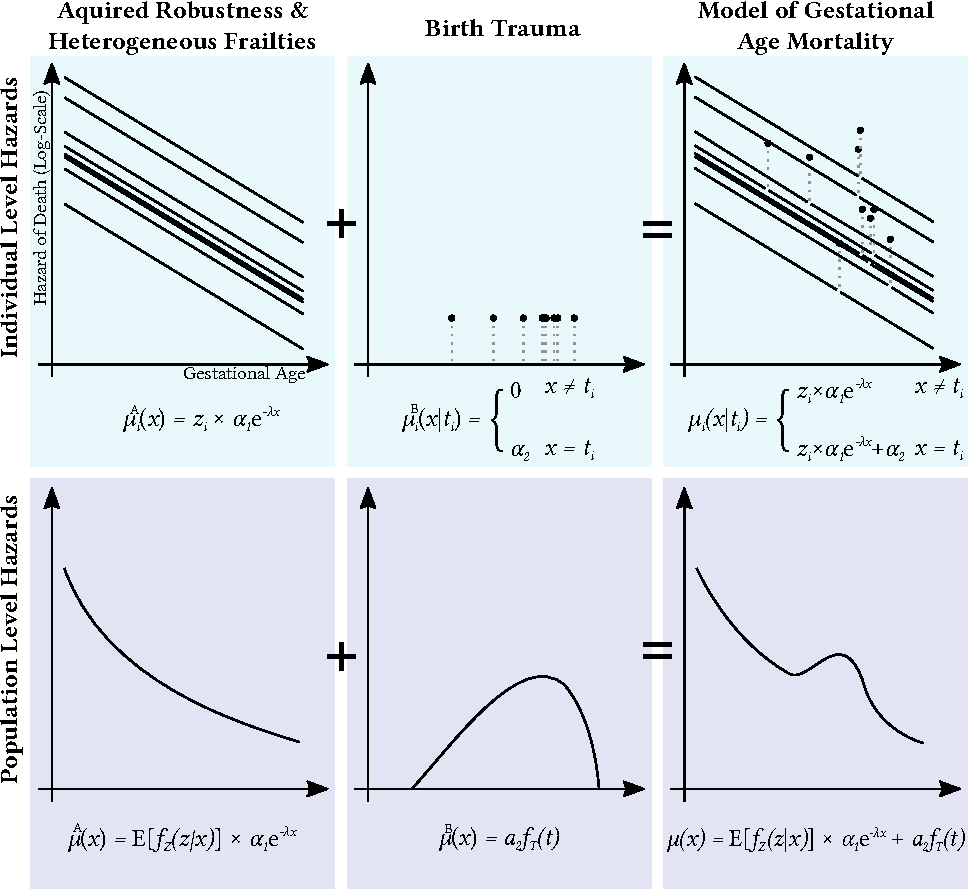
\includegraphics[width = \textwidth]{./fig/the_model.pdf}
  \caption{A model of mortality by gestational age for the developing human organism.}
  \label{fig:the_model}
\end{figure}


\section{Results} %%%%%%%%%%%%%%%%%%%%%%%%%%%%%%%%%%%%%%%%%%%%%%%%%%%%%%%%%%%%%
\label{sec:results}

Estimating the parameters of (\ref{eq:thelaw}) on the joint fetal-infant life table for the US conception cohort of 2009 yields a close fit with sensible parameter estimates (see figure \ref{fig:us_fimort_2009_mx_predobs}).

\begin{figure}[!htb]
  \centering
  \includegraphics[width = \textwidth]{./fig/us_fimort_2009_mx_predobs.pdf}
  \caption{The gestational age pattern of human mortality for US fetus and infants conceived in 2009. Lifetable mortality rates versus predicted hazard. Individual level data source: \cite{DVS2015}.}
  \label{fig:us_fimort_2009_mx_predobs}
\end{figure}

\section{Conclusion} %%%%%%%%%%%%%%%%%%%%%%%%%%%%%%%%%%%%%%%%%%%%%%%%%%%%%%%%
\label{sec:conclusion}

We have shown the gestational age pattern of human mortality from week 23 until week 100 after the last manse of the mother using a joint fetal-infant single decrement life table calculated from contemporary US micro-data on births, fetal- and infant deaths. To our best knowledge this is a novel approach of describing early mortality. The observed age pattern is remarkably regular and consistent with three hypotheses on the mechanics of \emph{ontogenescense}: 1) Acquired robustness: as the organism growths it becomes more resilient towards death, 2) birth trauma: the transition of birth is a stressful event and momentarily increases the force of mortality, 3) mortality selection: The frailest individuals die first, resulting in the mean force of mortality to decline with age.

We operationalized the three hypotheses by deriving a parametrized function capable of reproducing the observed gestational age pattern of human mortality. We assumed an ideal gestational age mortality trajectory for an individual comprised of acquired robustness and birth trauma and showed that the observed aggregated age pattern emerges out of heterogeneity in frailty and timing of labour between individuals.

While physicians and epidemiologists naturally separate fetal- from infant mortality we have presented evidence that both are indeed part of a \emph{mortality continuum} starting before birth and reaching into infancy. This holistic perspective might provide useful in studies on the plasticity of ontogenescense and early life mortality.

\clearpage

%%%% Bibliography %%%%%%%%%%%%%%%%%%%%%%%%%%%%%%%%%%%%%%%%%%%%%%%%%%%%%%%%%%%%%

\sloppy
\printbibliography

%\clearpage

%%%% Appendix %%%%%%%%%%%%%%%%%%%%%%%%%%%%%%%%%%%%%%%%%%%%%%%%%%%%%%%%%%%%%%%%%

% appendix figures follow A1, A2, B1... scheme
%\renewcommand\thefigure{\thesection.\arabic{figure}}
%\setcounter{figure}{0}

%\begin{appendix}
%\end{appendix}

\end{document}